\chapter{Arhitectura aplicației. Detalii}
În primul rând, \textbf{\thesistitle} este o aplicație de tipul utilitar, scopul acesteia este unul de uz intern, în cadrul facultății. Prin urmare, traficul efectuat de către utilizatori este unul scăzut, lucru ce permite o arhitectură monolitică.

În al doilea rând, arhitectura urmează un model \textit{MVC} (Model View Controller) caracteristic unei aplicații web de acest tip, unde clientul trimite anumite request-uri prin interacțiunea cu GUI-ul, iar serverul la rândul său transmite anumite informații. Acest model arhitectural permite o organizare și modularizare riguroasă a aplicației.

În al treilea rând, baza de date este una de tipul SQL deoarece este necesară stocarea unui număr relativ mare de relații între entități, reprezentate de către preferințele studenților. De aceea, a fost ales MySQL pentru modelarea relațiilor și datelor din aplicație.

Astfel, aplicația este pe trei niveluri (\textit{3-tier architecture}). Un nivel al clientului, \textit{Presentation Layer} ce facilitează utilizarea, un nivel de business, \textit{Application Layer}, ce tratează request-uri, efectuează operații de autentificare și autorizare, precum și algoritmice, iar în final un nivel de prelucrare al datelor, \textit{Data Layer}.

\begin{figure}[H]
	\centering
	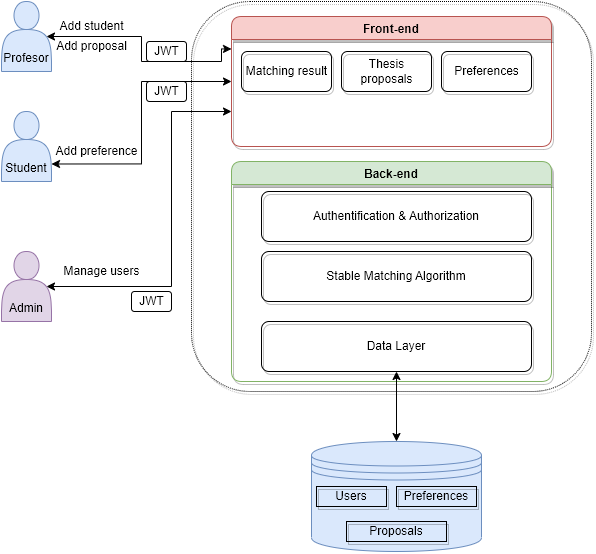
\includegraphics[width=\textwidth, left]{Thesis Matcher-App architecture.drawio.png}
	\caption{Arhitectura aplicației}
\end{figure}